\index{locks!problems with}
Conventionally, atomicity in shared-memory multiprocessors is provided
via mutual-exclusion \defn{locks} (see, for example,
\cite{Tanenbaum92}[p.~35]).  Although locks are easy to
implement using test-and-set, compare-and-swap, or
load-linked/{\bp}store-conditional instructions, they introduce a host of
difficulties.  To avoid deadlock when locking multiple objects, the
locks must be acquired in a consistent linear order, which makes
programming with locks error-prone and sometimes introduces
significant overheads in managing the lock acquisition protocol.
Moreover, locking can introduce other overheads, because a thread must
always grab a lock to gain exclusive access to a shared object,
regardless of whether another thread is actually attempting to access
the same object.

An alternative means of providing concurrency control is by the use of
\defn{transactions}.
A transaction can be thought of as a sequence of loads and stores
performed as part of a program which either
\defn{commits} or \defn{aborts}.  If a transaction
commits, then all of the loads and stores appear to have run
atomically with respect to other transactions.  That is, the
transaction's operations are not interleaved with those of other
transactions.  If a transaction aborts, then none of its stores take
effect and the transaction may be restarted, typically using a
backoff algorithm to preclude live-lock.

Although transactions can be implemented using mutual exclusion
(locks), our algorithms will utilize non-blocking synchronization
\index{non-blocking synchronization}
\cite{Lamport77,Herlihy88,HerlihyLuMo03,MassalinPu91,GreenwaldCh96} to
exploit optimistic concurrency among transactions.  Non-blocking
synchronization offers a number of advantages; foremost for the
concerns of this thesis is fault-tolerance.  A process which fails
while holding a lock within a critical region can prevent all other
non-failing processes from ever making progress.  It is in general not
possible to restore the locked data structures to a consistent state
after such a failure.  Non-blocking synchronization offers a graceful
solution to this trouble, as non-progress or failure of any one thread
will not affect the progress or consistency of other threads or the
system.

Implementing transactions using
non-blocking synchronization offers performance benefits as well.
Even in a failure-free system, page faults, cache misses, context
switches, I/O, and other unpredictable events may result in delays to the
entire system when mutual exclusion is used to guarantee the atomicity
of operation sequences; non-blocking
synchronization allows undelayed processes or processors to continue
to make progress.
Similarly, in real-time systems, the use of non-blocking
synchronization can prevent \defnlti{priority inversion} in the system
\cite{Jones97}, although na\"{\i}ve implementations may result in
starvation of low-priority tasks; see \charef{progress}.

The transaction model is a natural means to express both desired
atomicity and fault-tolerance properties.  In this thesis, I will also
show how transactions can be integrated into an object-oriented
language and used for fault-tolerance, backtracking,
exception-handling, and concurrency control in new programs.  I will
also show how
existing code might safely be ``transactified'' to fix existing
concurrency bugs (\charef{safe-transactify}).

I will present both software and hardware implementations of the
transaction model.
Previous implementation work has concentrated on the
\defni{transactional memory} abstraction
\cite{Knight86,HerlihyMo93,StoneStHe93,RajwarGo02,ShavitTo95,HerlihyLuMoSc03},
which has
been proposed as a general and flexible way to allow programs to read
and modify disparate primary memory locations atomically as a single
operation, much as a database transaction can atomically modify many
records on disk.

\index{HTM|see{Hardware Transactional Memory}}
\index{STM|see{Software Transactional Memory}}
\index{Hardware Transactional Memory}
\defn{Hardware transactional memory} (HTM) supports atomicity through
architectural means, whereas \defn{software transactional memory}
\index{Software Transactional Memory}
(STM) supports atomicity through languages, compilers, and libraries.
Researchers of both HTM and STM commonly express the opinion that
transactions need never touch many memory locations, and hence it is
reasonable to put a (small) bound on their size.  For HTM implementations,
they conclude that a small piece of additional hardware---typically in
the form of a fixed-size content-addressable memory and supporting
logic---should suffice.  For STM implementations, some researchers
argue additionally that transactions occur infrequently, and hence the
software overhead would be dwarfed by the other processing done by an
application.

In contrast, this thesis will assume that transactions may be of
arbitrary size and duration, and that details of the implementation
should not be exposed to the programmer of the system.  My goal is to
make concurrent and fault-tolerant programming easier, hopefully
without incurring much overhead in the process.  The target is
unbounded transactions because neither programmers nor compilers can
easily cope when an architecture imposes a hard limit on transaction
size.  An implementation might be optimized for transactions below a
certain size, but must still operate correctly for larger
transactions.  The size of transactional hardware should be an
implementation parameter, like cache size or memory size, which can
vary without affecting the portability of binaries.
\charef{hybrid} will show how a fast hardware implementation for
frequent short transactions can gracefully fail over to a software
implementation designed to efficiently execute large long-lived
transactions.

\section{Motivation}
\subsection{Four old things you can't (easily) do with locks}
%\section{Deadlocks, ordering, and other frightening prospects}

\subsubsection{Tweak performance with localized changes}
% global lock orders, oh my!
% usage rules embedded in comments
% races, lost wakeups
\subsubsection{Atomically move data between two thread-safe containers}
% locks don't compose
\subsubsection{Create a thread-safe double-ended queue}
% publishable result: michael/scott, 1996 PPoPP
\subsubsection{Handle asynchronous exceptions}

\subsection{Four new things transactions make easy}

I present three examples in this section, illustrating how
transactions can support fault-tolerance and back-tracking,
simplify locking, and provide a more intuitive
means for specifying thread-safety properties.
I will first examine a destructive traversal algorithm, showing how a
transaction implementation can be treated as an exception-handling
mechanism.   I then, using a network flow example, show how this
transaction mechanism can be used to simplify
the locking discipline required when synchronizing concurrent
modifications to multiple objects.
Finally, I show an existing race in the Java standard libraries (in 
the class \texttt{java.lang.StringBuffer}).  ``Transactification'' of
the existing class corrects this race.

\subsubsection{Destructive traversal}\label{sec:destruct}
Many recursive data structures can be traversed without the use of a
stack using pointer reversal.  This technique is widely used in
garbage collectors, and was first demonstrated in this context by
Schorr and Waite \cite{SchorrWa67}.  The following code implements a
pointer-reversal traversal of a simple singly-linked list:
\begin{inlinecode}
// destructive list traversal.
void traverse(List l) {
  List last = null, t;
  
  /* zip through the list, reversing links */
  for (int i=0; i<2; i++) {
    do {
      if (i==0) visit(l); // visit node
      t = l.next;
      l.next = last;
      last = l;
      l = t;
    } while (l!=null);
    l = last;
    // now do again, backwards. (restoring links)
  }
}
\end{inlinecode}

This function traverses the list, visiting nodes in order and then
reversing the {\tt next} pointer.  When the end of the list is
reached, the reversed links are traversed to restore the list's original
state.  

Of course, I've chosen the simplest possible data structure here, but
the technique works for trees and graphs---and the reader may mentally
substitute their favorite hairy update on a complicated data
structure.

In normal execution, the data structure is left complete and intact
after the operation.  But
imagine that an exception or fault occurs inside the {\tt visit()} method
at some point during the traversal: an assertion fires, an exception
occurs, the hardware hiccups, or a thread is killed.  Control may
leave the {\tt traverse()} method, but the data structure is left in
shambles.  What is needed is some exception-handling procedure to
restore the proper state of the list.  This can be manually coded with
Java's existing {\tt try}/{\tt catch} construct, but the
exception-handling code must be tightly-coupled to the traversal if it
is going to undo the list mutations.

\note{Used to have a try/catch with explicit fail in here.}
Instead, I can provide a non-deterministic choice operator,
{\tt try}/{\tt else}, and write the recovery code at a higher-level as:
\begin{inlinecode}
try {
  traverse(list);
} else { // try-else construct
  throw new Error();
}
\end{inlinecode}
\note{I'd prefer `fail t' here, but that raises the question of how
  to export objects from transactional contexts.}

The {\tt try}/{\tt else} block appears to make a non-deterministic
choice between executing the {\tt try} or the {\tt else} clause,
depending on whether the {\tt try} would succeed or not.
This can be straight-forwardly implemented
with a transaction around the traversal,
always initially attempting
the {\tt try}.  Exceptions or faults cause the transaction to abort;
when it does so all the
heap side-effects of the {\tt try} block disappear.

Introducing an explicit {\tt fail} statement allows us to use the same
{\tt try}/{\tt else} for back-tracking search.\index{back-tracking}
\note{Insert example here?}

\subsubsection{Network flow}\label{sec:flow}\index{network flow}

I'll turn our attention now to parallel codes.
Consider a serial program for computing network flow (see, for
example, \cite[Chapter 26]{CormenLeRi01}).  The inner loop of the code
pushes flow across an edge by increasing the ``excess flow'' on one
vertex and decreasing it by the same amount on another vertex.  One
might see the following Java code:
\begin{inlinecode}
void pushFlow(Vertex v1, Vertex v2, double flow) {
  v1.excess += flow; /* Move excess flow from v1 */
  v2.excess -= flow; /* to v2.                   */
}
\end{inlinecode}

To parallelize this code, one must preclude multiple threads from
modifying the excess flow on those two vertices at the same time.
Locks provide one way to enforce this mutual exclusion: 
\begin{inlinecode}
void pushFlow(Vertex v1, Vertex v2, double f) {
  Object lock1, lock2;
  if (v1.id < v2.id) {       /* Avoid deadlock. */
    lock1 = v1; lock2 = v2;
  } else {
    lock1 = v2; lock2 = v1;
  }
  synchronized(lock1) {
    synchronized(lock2) {
      v1.excess += f; /* Move excess flow from v1 */
      v2.excess -= f; /* to v2.                   */
    } /* unlock lock2 */
  } /* unlock lock1 */
}
\end{inlinecode}

This code is surprisingly complicated and slow compared to the
original.  Space for each object's lock must be reserved.
To avoid deadlock, the code must acquire the locks in
a consistent linear order, resulting in an unpredictable branch in the
code.  In the code shown,
I have required the programmer to insert an \texttt{id} field into
each vertex object to maintain a total ordering.
The time required to acquire the locks may be
an order of magnitude larger than the time to
modify the excess flow.
\note{Using FLEX, the locking code is over 11x
  slower than the no-locks code.  With Sun's JVM, this overhead falls
  to about 1.7x, because Sun is wicked smart about their lock
  implementations.}
What's more, all of this overhead is rarely
needed!  For a graph with thousands or millions of vertices, the
number of threads operating on the graph is likely to be less than a
hundred.  Consequently, the chances are quite small that two different
threads actually conflict.  Without the locks to implement mutual
exclusion, however, the program would occasionally fail.

Software transactions (and some language support) allow the
programmer to parallelize the original code using an \texttt{atomic}
keyword to indicate that the code block should appear to execute
atomically: 
\begin{inlinecode}
void pushFlow(Vertex v1, Vertex v2, double flow) {
  atomic { /* Transaction begin. */
    v1.excess += flow; /* Move excess flow from v1 */
    v2.excess -= flow; /* to v2.                   */
  } /* Transaction end. */
}
\end{inlinecode}

This {\tt atomic} region can be implemented as a transaction, and
with an appropriately non-blocking implementation, it
will scale better and execute faster than the locking version
\cite{AnanianAsKuLeLi04,HarrisFr03,GreenwaldCh96,MassalinPu91,HerlihyMo93,ShavitTo95}.
From the programmer's point of view, I've also eliminated the
convoluted locking protocol, which must
be observed rigorously everywhere the related fields are accessed if
deadlock and races are to be avoided.

Further, I can implement {\tt atomic} using the {\tt try}/{\tt else}
exception-handling mechanism I've already introduced:
\begin{inlinecode}
for (int b=0; ; b++) {
  try {
    // atomic actions
  } else {
    backOff(b);
    continue;
  }
  break; // success!
}
\end{inlinecode}

\note{How hard do I try to execute the {\tt try} block?}
I non-deterministically choose to execute the body of the {\tt
  atomic} block if and only if it will be observed by all to execute
atomically.  The same linguistic mechanism I introduced for
fault-tolerance and back-tracking provides atomic regions for
synchronization as well.
\note{Mention optimistic parallelism here?}

\subsubsection{The \texttt{StringBuffer} class}\label{sec:stringbuffer}
The existing \defni{monitor synchronization} methodology for Java
implicitly associates an 
lock with each object.  As in Java's progenitor, Emerald
\cite{BlackHuJuLe86,JulSt91},\index{Emerald}\footnote{See \charef{emerald}.}
data races are prevented by
requiring a thread to acquire an
object's lock before touching the object's shared fields.
However, the lack of races is not sufficient to prevent unanticipated
parallel behavior.

Flanagan and Qadeer \cite{FlanaganQa03} demonstrated this
insufficiency with an
actual bug they discovered in the Sun JDK 1.4.2 Java standard
libraries.  The \texttt{java.lang.StringBuffer}\index{java.lang.StringBuffer@\texttt{java.lang.StringBuffer}} class,
which implements a mutable string abstraction, is implemented as follows:
\begin{inlinecode}
public final class StringBuffer ... {
  private char value[];
  private int count;
  ... 
  public synchronized
  StringBuffer append(StringBuffer sb) {
    ...
A:  int len = sb.length();
    int newcount = count + len; 
    if (newcount > value.length)
      expandCapacity(newcount);
    // next statement may use stale len
B:  sb.getChars(0, len, value, count);
    count = newcount;
    return this;
  }
  public synchronized int length() { return count; }
  public synchronized void getChars(...) { ... }
}
\end{inlinecode}

The library documentation indicates that the methods of this class are meant
to execute atomically, and the {\tt synchronized} modifiers on the
methods are meant to accomplish this.

However, the {\tt append()} method is \emph{not} atomic.  Another
thread may change the length of the parameter \texttt{sb} (by adding
or removing characters) between the call to \texttt{sb.length()} at
label A and the call to \texttt{sb.getChars(\ldots)} at label B.
This non-atomicity may cause incorrect data to be appended to the
target or a \texttt{StringIndexOutOfBoundException} to be thrown. 
Although the calls to
\texttt{sb.length()} and \texttt{sb.getChars()} are individually
atomic, they do not compose to form an atomic implementation of
\texttt{append()}.  
%The simple monitor synchronization scheme breaks
%down when operations touch multiple objects.

Note that replacing {\tt synchronized} with {\tt atomic} in
this code gives us the semantics
we desire: the atomicity of nested {\tt atomic} blocks is guaranteed
by the atomicity of the outermost block, ensuring that the entire
operation appears atomic.

Both the network flow example and this {\tt StringBuffer} example require
synchronization of
changes to more than one object.
Monitor synchronization is not
well-suited to this task.  Atomic regions implemented with
transactions can be used to simplify the locking discipline required
to synchronize multi-object mutation
and provide a more intuitive specification for the desired
concurrent properties.  Further, the {\tt StringBuffer} example shows
that simply replacing {\tt synchronized} with {\tt atomic} provides a
alternative semantics which may in fact correct existing
synchronization errors.
For many Java programs, the
semantics of {\tt atomic} and {\tt synchronized} are identical; see
\charef{semantic}.
\note{Can I make this rigorous?}

\subsection{Some things we still can't (easily) do}\label{sec:xlimit}
The transaction mechanism presented here is not a universal
replacement for all synchronization.  In particular, transactions
cannot replace blocking producer-consumer queues and mutual exclusion
required to serialize I/O, although the needed locks can certainly be
built with transactions.  Integrating I/O within a transactional
context remains poorly understood.  However, large programs---the
Linux kernel, for example---have been written such that locks are
never held across context switches or I/O operations.  Transactions
provide a complete solution for this limited synchronization.
One of the goals of this thesis is to investigate better integration
of transactional with inherently non-transactional operations.
One promising approach is the addition of explicit ``recovery'' blocks
to undo the effects of non-transactional regions embedded within
an aborting transaction.

\section{Finding transactions}\label{sec:auto}
One of the difficulties of proposing a novel language feature is the
lack of benchmarks for its evaluation.  Although there is no body of
code yet using {\tt atomic} regions, there is a substantial body of
code which uses Java (locking) synchronization.  This thesis will
utilize the Flex compiler to
substitute {\tt atomic} blocks (methods) for {\tt
  synchronized} blocks (methods) in order to evaluate the properties
Java transactions are likely to have.  Note that the semantics are not
precisely compatible: the existing \indexed{Java memory model} allows
unsynchronized updates to shared fields to be observed within a
synchronized block, while such updates will never be visible to an
{\tt atomic} block.  The proposed revision of the Java memory model
\cite{MansonPu02} narrows the semantic gap, however I do not
plan to treat {\tt volatile} fields in this work.  See
\charef{semantic} for more details.

Despite the differences in semantics, the automatic substitution of
{\tt atomic} for {\tt synchronized} does, in fact, preserve the
correctness of the benchmarks I've examined.  Moreover, as
mentioned in \charef{stringbuffer}, it
fixes the synchronization issue with {\tt java.lang.StringBuffer}.

One goal of this thesis is to make such improperly synchronized
applications correct and race-free, in effect fixing certain common
synchronization errors.  To this effect, I need to preserve the
correct operation of {\tt atomic} even in the face of unsynchronized
accesses from outside the {\tt atomic} block to the fields used within
it.  Imagine unsynchronized code directly altering the length field of
{\tt StringBuffer}.  This should not cause the {\tt atomic}
{\tt StringBuffer.append()} method to appear non-atomic.
Some existing work on software transaction systems \cite{HarrisFr03}
does not support this style of operation.

\label{sec:properties}
The initial results of this thesis
explore the implications of exposing the transaction
mechanism to user-level code through a compiler.
I compiled the SPECjvm98 benchmark suite with the FLEX Java compiler
\cite{Flex},
modified to turn synchronized blocks and methods into transactions,
in order to investigate the properties of the transactions in such
``automatically converted'' code.
Method splitting was performed to distinguish methods called from
within an atomic block, and nested
\texttt{atomic} blocks were implemented as a single
transaction around the outermost \texttt{atomic} region.  I
instrumented this transformed program to produce a trace of
memory references and transaction boundaries for analysis.
I found both large
transactions (touching up to 8.9 million cache lines) and frequent
transactions (up to 45 million of them).

The SPECjvm98 benchmark suite represents a variety of typical Java
applications which use the capabilities of the Java standard library.
Although the SPECjvm98 benchmarks are largely single-threaded, since
they use the thread-safe Java standard libraries they contain
synchronized code which is transformed into transactions.  Because in
this evaluation I am looking at transaction properties only, the
multithreaded \texttt{227\_mtrt} benchmark is identical to its
serialization, \texttt{205\_raytrace}.  For consistency, I present
only the latter.

\begin{figure}\sis%
\begin{center}
\begin{tabular}{lrrrr}
        & total      &              & transactional & biggest\\
program & memory ops & transactions & memory ops    & transaction \\\hline
{\tt 201\_compress} & 2,981,777,890 & 2,272 & $<$0.1\% & 2,302 \\
{\tt 202\_jess} & 405,153,255 & 4,892,829 & 9.1\% & 7,092 \\
{\tt 205\_raytrace} & 420,005,763 & 4,177 & 1.7\% & 7,149,099 \\
{\tt 209\_db} & 848,082,597 & 45,222,742 & 23.0\% & 498,349 \\
{\tt 213\_javac} & 472,416,129 & 668 & 99.9\% & 118,041,685 \\
{\tt 222\_mpegaudio} & 2,620,818,169 & 2,991 & $<$0.1\% & 2,281 \\
{\tt 228\_jack} & 187,029,744 & 12,017,041 & 34.2\% & 14,266 \\
\end{tabular}
\end{center}
\caption[Transactification of SPECjvm98 benchmark suite.]%
 {Transactification of SPECjvm98 benchmark suite: resulting
  transaction counts and sizes, compared to total number of memory
  operations (loads and stores).  These are full input size runs.
}\label{fig:perfnums}
\end{figure}
\figput{tr-quad}{Classification of SPECjvm98 benchmarks into quadrants
based on transaction properties.}

\figref{perfnums} shows the raw sizes and frequency of transactions in
the transactified SPECjvm98 suite.
\figref{tr-quad} proposes a
taxonomy for Java applications with transactions, grouping the SPECjvm98
applications into quadrants based on the number and size of the
transactions which they perform.  Applications in Quads II and IV
require an efficient transaction implementation, because they contain
many transactional operations.
Quads III and IV contain at least some very large transactions, which
pose difficulties for currently-proposed hardware transactional memory
schemes.  We will now
examine the benchmarks in each quadrant to determine why its program
logic caused it to be classified in that quadrant.

Quad I applications perform few (up to about 2000) small
transactions.  These applications include \texttt{201\_compress}, an
implementation of gzip compression, and \texttt{222\_mpegaudio}, an
MP3 decoder.  Both of these applications perform inherently serial
tasks.  They perform quite well with locks, and would likely execute
with acceptable performance even with a na\"\i{}ve software
implementation of transactions, as long as the impact on
non-transactional operations was minimal.

Quad II applications perform a large number of small transactions.
The expert system \texttt{202\_jess} falls in this category, as do
small input sizes of \texttt{209\_db}, a database.  These benchmarks
perform at least an order of magnitude more transactions than Quad
I applications, and all of the transactions are small enough to 
comfortably fit the known hardware transactional memory schemes, if
one were to be implemented.

Quad III includes \texttt{205\_raytrace}, a ray-tracing renderer.  A
small number of transactions are performed, but they may grow very
large.  Existing bounded hardware transactional schemes will not
suffice.  The large
transactions may account for a large percentage of total memory
operations, which may make software schemes impractical.

Finally, Quad IV applications such as \texttt{209\_db} and the
\texttt{213\_javac} Java compiler application perform a large number
of transactional memory operations with at least a few large transactions.  

The \texttt{213\_javac} Java compiler application and the large input
size of the \texttt{209\_db} benchmark illustrate that some programs
contain \emph{extremely} large transactions.  When \texttt{213\_javac}
is run on its full input set, it contains 4 very large transactions,
each of which contains over 118 million transactional memory
operations.  Closer
examination reveals that the method \texttt{Javac.compile()}, which
implements the entire compilation process, is marked as synchronized:
the programmer has explicitly requested that the entire compilation
occur atomically.

The \texttt{209\_db} benchmark suffers from a similar problem: at one
point the benchmark atomically scans an index vector and removes an
element, creating a potentially large transaction if the index is
large.  The size of this index is correlated in these benchmarks with
the input size, but it need not be: a large input could still result
in a small index, and (to some degree) vice-versa.

A similar situation arises in the {\tt java.lang.StringBuffer} code
shown in \ref{sec:stringbuffer}:  a call to the synchronized
\texttt{sb.getChars()} method means that
the size of the transaction for this method will grow like the length
of the parameter~\texttt{sb}.  In other words, the transaction can be
made arbitrarily large by increasing the length of \texttt{sb}; or,
equivalently, there is no bound on transaction size without a bound on
the size of the string~\texttt{sb}.

\epsfigput[Distribution of transaction size in the SPECjvm98 benchmark
  suite.]{tr-sz-all}{Distribution of transaction size in the
  SPECjvm98 benchmark suite.  Note that the x-axis uses a logarithmic
  scale.}

Any scheme which allows the programmer free reign over specifying
desired transaction and/or atomicity properties will inevitably result
in some applications in each of these categories.  As existing
hardware transactional memory schemes only handle applications in Quad
I or II, they are not a good implementation technique for a general
language mechanism.  \figref{tr-sz-all} restates this problem, by
illustrating the distribution of transaction sizes in these
applications on a semi-log scale.

\punt{
\vspace*{2mm}
\begin{figure}\sis%
\begin{center}
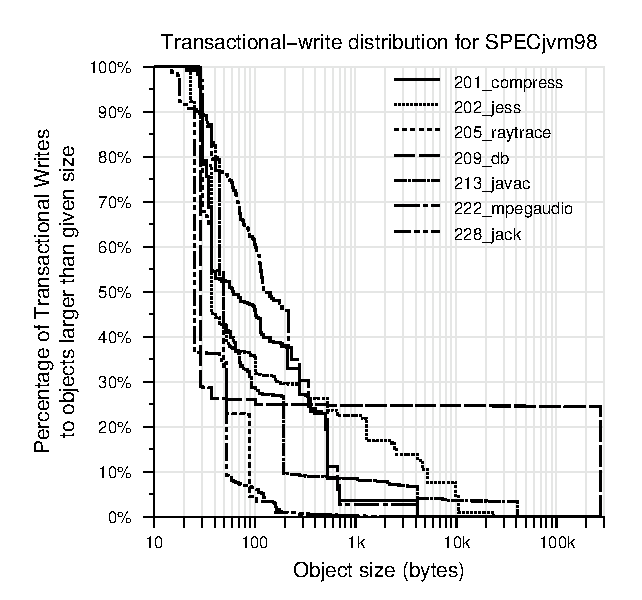
\includegraphics[width=2.25in,clip=true]{Figures/tr-w-all.eps}%
~~~~~%
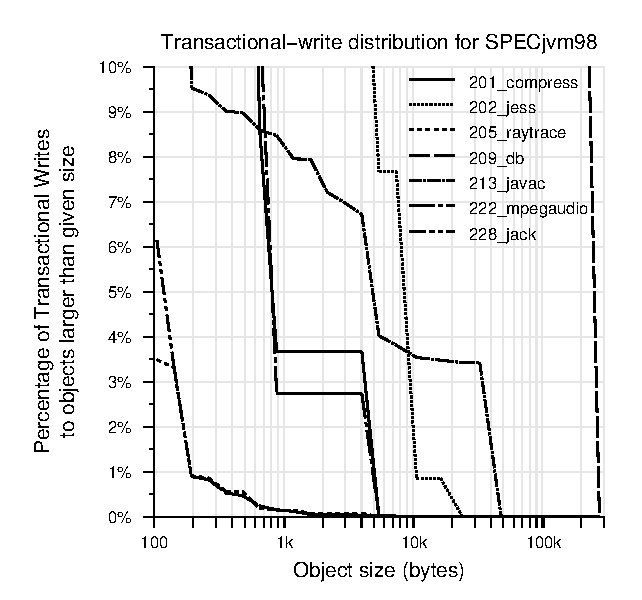
\includegraphics[width=2.25in,clip=true]{Figures/tr-w-ten.eps}%
\end{center}%
\caption{Proportion of transactional writes to objects equal to or
  smaller than a given size.  The right-hand graph zooms in on a
  portion of the relation shown in the left; note in particular that
  y-axis full-scale is only 10\% in the right-hand graph.}%
\label{fig:tr-w}%
\end{figure}%
Our software transactions implementation clones objects on
transactional writes, so that the previous state of the object can be
restored if the transaction aborts.  With this in mind, I was
interested in the number of writes to \emph{large} objects, or,
equivalently, on the object size distribution of transactional
writes.  \figref{tr-w} shows this distribution for the SPECjvm98
applications. 
}

\vspace*{5mm}

These initial results show that real applications can be
transactified with modest effort, yielding significant gains in
concurrency.  In other work \cite{AnanianAsKuLeLi04} we have shown
that a factor of 4 increase in concurrency can be obtained
by doing nothing more than converting locks to transactions.  Since
the transactified applications may contain large transactions,
proposed hardware support for transactions is inadequate.

%%%%%%%%%%%%%%%%%%%%%%%%%%%%%%%%%%%%%%%%%%%%%%%%%%%%%%%%%%%%%%%%%%
\section{Related work}\label{sec:related}

A number of researchers have been investigating transactional memory
systems.  This thesis will be the first to present a hybrid hardware/software
model-checked non-blocking
object-oriented system which allows co-existence of non-transactional and
transactional accesses to a dynamic set of object fields.

\subsection{Non-blocking synchronization}\label{sec:nb-sync}

Lamport presented the first alternative to synchronization via mutual
exclusion in \cite{Lamport77}, for a limited situation involving a single
writer and multiple readers.  Lamport's technique relies on reading
guard elements in an order opposite to that in which they are written,
guaranteeing that a consistent data snapshot can be recognized.  The
writer always completes its part of the algorithm in a constant number
of steps; readers are guaranteed to complete only in the absence of
concurrent writes.

Herlihy formalized \emph{wait-free} implementations of
concurrent data objects in \cite{Herlihy88}.  A wait-free implementation
guarantees that any process can complete any operation in a finite
number of steps, regardless of the activities of other processes.
Lamport's algorithm is not wait-free
because readers can be delayed indefinitely.

Massalin and Pu introduced the term \emph{lock-free} to describe 
algorithms with weaker progress guarantees.
A lock-free implementation guarantees only that \emph{some}
process will complete in a finite number of steps
\cite{MassalinPu91}.  Unlike a wait-free implementation,
lock-freedom allows starvation.  Since other simple techniques can be
layered to prevent starvation (for example, exponential backoff),
simple lock-free implementations are usually seen as worthwhile practical
alternatives to more complex wait-free implementations.

An even weaker criterion, \emph{obstruction-freedom}, was introduced
by Herlihy, Luchangco, and Moir in \cite{HerlihyLuMo03}.
Obstruction-freedom only guarantees progress for threads executing in
isolation; that is, although other threads may have partially
completed operations, no other thread may take a step until the
isolated thread completes.  Obstruction-freedom not only allows
starvation of a particular thread, it allows contention among threads
to halt all progress in all threads
indefinitely.  External mechanisms are used to reduce contention
(thus, achieve progress) including backoff, queueing, or timestamping.

We will use the term \emph{non-blocking} to describe
generally any synchronization mechanism which doesn't rely on mutual
exclusion or locking, including wait-free, lock-free,
and obstruction-free implementations.
We will be concerned mainly with lock-free algorithms.%
\footnote{Note that some authors use ``non-blocking'' and
  ``lock-free'' as synonyms, usually meaning what we here call
  \emph{lock-free}.  Others exchange our definitions for ``lock-free''
  and ``non-blocking'', using lock-free as a generic term and non-blocking
  to describe a specific class of implementations.  As there is
  variation in the field, we choose to use the parallel construction
  \emph{wait-free}, \emph{lock-free}, and \emph{obstruction-free} for
  our three specific progress criteria, and the dissimilar
  \emph{non-blocking} for the general class.}

\subsection{Efficiency}\label{sec:efficiency}
Herlihy presented the first \emph{universal} method for wait-free
concurrent implementation of an arbitrary sequential object
\cite{Herlihy88,Herlihy91}.  This original method was based on
a \emph{fetch-and-cons} primitive, which atomically places
an item on the head of a list and returns the list of items following
it; all concurrent primitives capable of solving the
$n$-process consensus problem---\emph{universal} primitives---were
shown powerful enough to implement \emph{fetch-and-cons}.
In Herlihy's method, 
every sequential operation is translated into two steps.  In the first,
\emph{fetch-and-cons} is used to place the name and arguments of the
operation to be performed
at the head of a list, returning the other operations on the list.
Since the state
of a deterministic object is completely determined by the history of
operations performed on it, applying the operations returned
in order from last to first is sufficient to locally reconstruct the
object state 
prior to our operation.
We then use the prior state to compute the result of our operation
without requiring further synchronization with the other processes.

This first universal method was not very practical, a shortcoming
which Herlihy soon addressed \cite{Herlihy93}.  In addition, his revised universal
method can be made lock-free, rather than wait-free, resulting in
improved performance.  In the lock-free version of this method,
objects contain a shared variable
holding a pointer to their current state.  Processes begin by loading
the current state pointer and then copying the referenced state to a
local copy.  The sequential operation is performed on the
copy, and then if the object's shared state pointer is unchanged from
its initial load it is atomically swung to point at the updated state.

Herlihy called this the ``small object protocol'' because the object
copying overhead is prohibitive unless the object is small enough to
be copied efficiently (in, say, $O(1)$ time).  He also presented a
``large object protocol'' which requires the programmer to
manually break the object into small blocks, after which the small
object protocol can be employed. 
[This trouble with large objects is
common to many non-blocking implementations; our solution is presented
in \charef{largeobj}.]

Barnes provided the first universal non-blocking implementation
method which avoids object copying \cite{Barnes93}.  He eliminates the
need to store ``old'' object
state in case of operation failure by having all threads cooperate to
apply operations.  For example, if the first processor begins an operation
and then halts, another processor will complete the operation of the first
before applying its own.  Barnes proposes to accomplish the
cooperation by creating a parallel state machine for each operation,
so that each thread can independently try to advance the machine from state
to state and thus advance incomplete operations.%
\footnote{It is interesting to note that Barnes' cooperative method
  for non-blocking 
  situation plays out in a real-time system very similarly to priority
  inheritance for locking synchronization.}
Although this avoids
copying state, the lock-step cooperative process is extremely
cumbersome and does not appear to have ever been implemented.
Furthermore, it does not protect against errors in the implementation
of the operations, which could cause \emph{every} thread to fail in turn
as one by one they attempt to execute a buggy operation.

Alemany and Felten \cite{AlemanyFe92} identified two factors hindering the
performance of non-blocking algorithms to date: resources wasted by operations
that fail, and the cost of data copying.  Unfortunately, they
proceeded to
``solve'' these problems by ignoring short delays and failures and
using operating system support to handle delays caused by
context switches, page faults, and
I/O operations.  This works in some situations, but obviously suffers
from a bootstrapping problem as the means to implement an operating system.

Although lock-free implementations are usually assumed to be more
efficient that wait-free implementations, LaMarca \cite{LaMarca94}
showed experimental evidence that Herlihy's simple
wait-free protocol scales very well on parallel machines.
When more than about twenty threads are involved, the wait-free
protocol becomes
faster than Herlihy's lock-free small-object protocol, three OS-aided
protocols of LaMarca and Alemany and Felten, and a
\emph{test-and-Compare\&Swap} spin-lock.

% Afek et al have a somewhat complicated improved wait-free method.

% Transactional memories?
\subsection{Transactional Memory systems}\label{sec:tm}

Transactions are described in the database context by Gray
\cite{Gray81b}, and \cite{GrayRe93} contains a thorough treatment of
database issues.  Hardware Transactional Memory (HTM) was first
proposed by Knight~\cite{Knight86},
and Herlihy and Moss coined the term ``transactional memory'' and
proposed HTM in the context of lock-free data
structures~\cite{HerlihyMo92,HerlihyMo93}.  The BBN
Pluribus~\cite[Ch.~23]{SiewiorekBeNe82} provided transactions, with an
architectural limit on the size of a transaction.  Experience with
Pluribus showed that the headaches of programming correctly with such
limits can be at least as challenging as using locks.  The
\defn{Oklahoma Update} is another variation on transactional
operations with an architectural limit on the number of values in a
transaction~\cite{StoneStHe93}.

Transactional memory is sometimes described as an extension of
Load-Linked/Store-Conditional \cite{JensenHaBr87} and other atomic
instruction sequences.  In fact, some CISC machines, such as the VAX,
had complex atomic instructions such as enqueue and
dequeue~\cite{Digital96}.

Of particular relevance are \defn{Speculative Lock
Elision} (SLE) \cite{RajwarGo01} and \defn{Transactional Lock Removal}
(TLR) \cite{RajwarGo02}, which speculatively identify locks and use
the cache to give the appearance of atomicity.  SLE and TLR handle
mutual exclusion through a standard programmer interface (locks),
dynamically translating locks into transactional regions.  My
research thrust differs from theirs in that I hope to free
programmers from the protocol complexities of locking, not just
optimize existing practice.  The quantitative results presented in
this thesis confirm their finding that transactional hardware can be
more efficient than locks.

Martinez and Torrellas proposed \defn{Speculative Synchronization}
\cite{MartinezTo02}, which allows some threads to execute atomic
regions of code speculatively, using locks, while guaranteeing forward
progress by maintaining a nonspeculative thread.  These techniques
gain many of the performance advantages of transactional memory, but
they still require new code to obey a locking protocol to avoid
deadlock.

The recent work on \defn{Transactional memory Coherence and
Consistency} (TCC)~\cite{HammondWoCh04} is also relevant to our work.
TCC uses a broadcast bus to implement the transaction protocols,
performing all the writes of a particular transaction in one atomic
bus operation.  This strategy limits scalability, whereas both the UTM and
LTM proposals in \charef{hardimpl}
can employ scalable cache-consistency protocols to implement
transactions.  TCC affirms the conclusion we draw from our own
\figref{tr-sz-all}: most transactions are small, but some are very large.  TCC
supports large transactions by locking the broadcast bus and stalling
all other processors when any processor buffer overflows, whereas UTM
and LTM allow overlapped execution of multiple large transactions with
local overflow buffers.  TCC is similar to LTM in that transactions
are bound to processor state and cannot extend across page faults,
timer interrupts, or thread migrations.

\note{Insert VTM reference here \cite{RajwarHeLa05}.}

Several software transaction systems have been proposed.  Some constrain the
programmer and make transactions difficult to use.  All have
relatively high overheads, which make transactions unattractive for
uniprocessor and small SMP systems. [Once the number of processors is
large enough, the increased parallelism which can be provided by
optimistic transactions may cancel out the performance penalty of
their use.]

The first proposal for software transactional memory was proposed by
Shavit and Touitou \cite{ShavitTo95}; their system requires that all
input and output locations touched by a transaction be known in
advance, which limits its application.  It performs at least 10
fetches and 4 stores per location accessed (not counting the loads and
stores directly required by the computation).  The benchmarks
presented were run on between 10 and 64 processors.

Rudys and Wallach \cite{RudysWa02} proposed a copying-based
transaction system to allow rollback of hostile codelets.
They show an order of magnitude slowdown for field and array
accesses, and 6x to 23x slowdown on their benchmarks.

Herlihy, Luchango, Moss, and Scherer's scheme \cite{HerlihyLuMoSc03}
allows transactions to touch a dynamic set of memory locations;
however the user still has to explicitly \emph{open} every object touched
before it can be used in a transaction.  This implementation is based
on object copying, and so has poor performance for large objects and
arrays.  Not including work necessary to copy objects involved in
writes, they require $O(R(R+W))$ work to open $R$ objects for reading
and $W$ objects for writing, which may be quadratic in the number of objects
involved in the transaction.   A list insertion benchmark which they
present shows 9x slowdown over a locking scheme, although they beat the locking
implementation when more than 5-10 processors are active.  They
present benchmark data with up to 576 threads on 72 processors.

Harris and Fraser built a software transaction system on a flat
word-oriented transactional memory abstraction \cite{HarrisFr03},
roughly similar to simulating Herlihy's original hardware
transactional memory proposal in software.  This avoids problems with
large objects.  Performing $m$ memory operations touching $l$ distinct
locations costs at least $m+l$ extra reads and $l+1$ CAS operations, in
addition to the reads and writes required by the computation.
They appear to execute about twice as slowly as a locking
implementation on some microbenchmarks.  They benchmark on a
4-processor as well as a 106-processor machine; their crossover point
(at which the blocking overhead of locks matches the software
transaction overhead) is around 4 processors.
Note that Harris and Fraser do not address the problem of
concurrent non-transactional operations on locations involved in a
transaction.  Java synchronization allows such concurrent operations,
with semantics given by the Java memory model \cite{MansonPu02}.
We support these operations safely using the mechanisms presented in
\charef{softimpl}.

Programmers will be reluctant to use transactions to synchronize their
code when it results in their code running more slowly on the uniprocessor
and small-SMP systems which are most common today.

Herlihy and Moss \cite{HerlihyMo93} suggested that small transactions
might be handled in cache with overflows handled by software.  These
software overflows must interact with the transactional hardware in
the same way that the hardware interacts with itself, however.
In \charef{hybrid} we present just such a system.


%%%%%%%%%%%%%%%%%%%%%%%%%%%%%%%%%%%%%%%%%%%%%%%%
\subsection{Language-level approaches to synchronization}
\begin{figure}
{\samepage\it\sis%
\begin{tabular}{l}%
{\bf const} myDirectory == {\bf object} oneEntryDirectory\\
~~{\bf export} Store, Lookup\\
~~{\bf monitor}\\
~~~~{\bf var} name : String\\
~~~~{\bf var} AnObject : Any\\
\\
~~~~{\bf operation} Store [ n : String, o : Any ]\\
~~~~~~name $\gets$ n\\
~~~~~~AnObject $\gets$ o\\
~~~~{\bf end} Store
\\
~~~~{\bf function} Lookup [ n : String ] $\to$ [ o : Any ]\\
~~~~~~{\bf if} n = name\\
~~~~~~~~{\bf then} o $\gets$ AnObject\\
~~~~~~~~{\bf else} o $\gets$ {\bf nil}\\
~~~~~~{\bf end if}\\
~~~~{\bf end} Lookup\\
\\
~~~~{\bf initially}\\
~~~~~~name $\gets$ {\bf nil}\\
~~~~~~AnObject $\gets$ {\bf nil}\\
~~~~{\bf end initially}\\
\\
~~{\bf end monitor}\\
{\bf end} oneEntryDirectory
\end{tabular}
}
\caption{A directory object in Emerald, from \cite{BlackHuJuLe86},
  illustrating the use of monitor synchronization.\index{monitor synchronization}}
\label{fig:emerald-dir}
\end{figure}

\begin{figure}
{\ttfamily\sis\small%
\begin{tabular}{l}
class Account \{\\
\\
~~int balance = 0;\\
\\
~~{\bf atomic} int deposit(int amt) \{\\
~~~~int t = this.balance;\\
~~~~t = t + amt;\\
~~~~this.balance = t;\\
~~~~return t;\\
~~\}\\
\\
~~{\bf atomic} int readBalance() \{\\
~~~~return this.balance;\\
~~\}\\
\\
~~{\bf atomic} int withdraw(int amt) \{\\
~~~~int t = this.balance;\\
~~~~t = t - amt;\\
~~~~this.balance = t;\\
~~~~return t;\\
~~\}\\
\\
\}\\
\end{tabular}
}\vspace{.2in}
\caption{A simple bank account object, adapted from \cite{FlanaganQa03},
  illustrating the use of the \atomic modifier.}
\label{fig:atomic}
\end{figure}

Our work on integrating transactions into the Java programming
language is related to prior work on integrating synchronization
mechanisms for multiprogramming, and in particular, to prior work on
synchronization in an object-oriented framework.

\index{Emerald|(}\label{sec:emerald}
The Emerald system \cite{BlackHuJuLe86,JulSt91} introduced
\defnlti{monitored objects} for synchronization.  Emerald code to
implement a simple directory object is shown in
Figure~\ref{fig:emerald-dir}.  Each object is associated with
Hoare-style monitor, which provides mutual exclusion and process
signalling.  Each Emerald object is divided into a monitored part and
a non-monitored part.  Variables declared in the monitored part are
shared, and access to them from methods in the non-monitored part is
prohibited---although non-monitored methods may call monitored methods
to effect the access.  Methods in the monitored part acquire the monitor lock
associated with the receiver object before entry and release it on
exit, providing for mutual exclusion and safe update of the shared
variables.  Monitored objects naturally integrate synchronization into
the object model.

Unlike Emerald monitored objects, where methods can only acquire the
monitor of their receiver and where restricted access to shared
variables is enforced by the compiler, Java implements a loose
variant where any monitor may be explicitly acquired and no shared
variable protection exists.  As a default, however, Java methods
declared with the {\tt synchronized} keyword behave like Emerald
monitored methods,
ensuring that the monitor lock of their receiver is held during execution.

Java's synchronization primitives arguably allow for more efficient
concurrent code than Emerald's---for example, Java objects can use
multiple locks to
protect disjoint sets of fields, and coarse-grain locks can be used
which protect multiple objects---but Java is also more prone to programmer
error.  However, even Emerald's restrictive
monitored objects are not sufficient to prevent data races.  As a
simple example, imagine that an object provided two monitored methods
{\tt read} and {\tt write} which accessed a shared variable.
Non-monitored code can call {\tt read}, increment the value returned,
and then call {\tt write}, creating a classic race condition scenario.
The atomicity of the parts is not sufficient to guarantee atomicity of
the whole \cite{FlanaganQa03}.
\note{``Composibility'': cite PPoPP paper \cite{HarrisMaPeHe05}?}
\index{Emerald|)}

This suggests that a better model for synchronization in
object-oriented systems is \defnlti{atomicity}.  Figure~\ref{fig:atomic}
shows Java extended with an \atomic keyword to implement an
object representing a bank account.  Rather than explicitly
synchronizing on locks, I simply require that the methods marked
\atomic execute atomically with respect to other threads in the
system; that is, that every execution of the program computes the same
result as some execution where all atomic methods were run \emph{in
  isolation} at a certain point in time, called the
\defni{linearization point}, between their invocation and return.
Note that
atomic methods invoked directly or indirectly from an atomic
method are subsumed by it: if the outermost method appears atomic,
then by definition all inner method invocations will also appear atomic.
Flanagan and Qadeer provide a more formal semantics in \cite{FlanaganQa03}.
Atomic methods can be analyzed using sequential reasoning techniques, which
significantly simplifies reasoning about program correctness.

Atomic methods can be implemented using locks.  A simple if inefficient
implementation would simply acquire a single global lock during
the execution of every atomic method.  Flanagan and Qadeer
\cite{FlanaganQa03} present a more sophisticated technique which proves that
a given implementation using standard Java monitors correctly
guarantees method atomicity.

The transaction implementations presented in this thesis will use
non-blocking synchronization to implement atomic methods.

